\documentclass{article}
\usepackage[utf8]{inputenc}

\usepackage{authblk}
\usepackage{multicol}
%\usepackage{natbib}
\usepackage{graphicx}
\usepackage{abstract}
\usepackage{float}
\usepackage[english]{babel}
\usepackage{amsmath}
\usepackage{subfigure}
\usepackage{alltt}
\usepackage{url}
\usepackage{multirow}
\usepackage[margin=3cm]{geometry}



\title{Human Connectomics Visualization: Techniques and Methodologies}
\author{Giorgio Conte}
%\date{December, $11^{th}$ 2014}
\affil{Creative Coding Research Group\\ Department of Computer Science\\University of Illinois at Chicago}



\begin{document}

\maketitle
\begin{abstract}
Studies in understanding how brain's regions are inter-connected is recently becoming more and more popular. Thanks to the advances in non-invasive neuroimaging technologies, such as functional Magnetic Resonance Imaging (fMRI) and Diffusion Tensor Imaging (DTI), large dataset can also be collected from living subjects. Thus, the need of visual analytic tools able to deal with this data is becoming a priority for neuroscientists. This work aims at surveying the main visualization techniques and methodologies already present in the academic literature as well as the new trends are taking place in this field. The main phenomena we are witnessing is a transition from stand-alone, local 2D visualization tools to more flexible and cross-platforms web-based applications which exploit 3D rendering.
\end{abstract}

\begin{multicols}{2}
\raggedcolumns

\section{Introduction}
\label{sec:introduction}

Being able to deeply understand how the brain is connected is one of the main challenges in the last years among neuroscientists. With the advent and the refinement of new technologies like \textit{functional Magnetic Resonance Imaging} (fMRI) and \textit{Diffusion Tensor Imaging}, also addressed as \textit{diffusion Magnetic Resonance Imaging} (diffusion MRI), experts are able to collect and derive data about how brain's regions are inter-connected. Very frequently the map of neural connections is addressed as \textit{connector} or \textit{human connectomics}.\\
Visualizing these data in an effective way would allow people to navigate and explore all the wired connections that are in the brain. Moreover, thanks to this kind of visualizations is possible to understand better the different interconnection patterns between healthy subjects and other people who suffer from a wide range of neuropsychiatric illnesses like bipolar, body dysmorphic disorder, schizophrenia, Alzheimer's disease and late-life depression. \\
Many visualization tools have been proposed in the academic literature, however the vast majority of them perform 2D visualizations and, since this research field is quite novel, there is still room for improvement.
The aim of this work is to report and survey the visualizations tools already present in the academic literature as well as to outline the new trends for the near future.\\
The paper is structured as follows. In section \ref{sec:domain} there is a more detailed introduction about the human Connectome. Then, a detailed list of common tasks is presented in section \ref{sec:mainTasks}, while in section \ref{sec:survey} I describe accurately the most interesting tools already present in the literature. In section \ref{sec:futureWorks} future works and some possibly newer trends are reported. Finally, in section \ref{sec:conclusions} I draw some conclusions.

%-------------------------------------------------------------------------

\section{Domain}
\label{sec:domain}

The human brain's connectome has been always considered by neuroscientists a very interesting and challenging topic. However, it is only in the last few ten years, when more powerful and more accurate technologies took place firmly in the research area, that more detailed studies have been conducted. Moreover, thanks to new technologies it is now possible to get data from living human subject, that is why they are also addressed as \textit{in vivo} techniques. In fact, through very advanced procedures and algorithms, experts can collect data about the functional and structural connectivity of the brain \textit{in vivo}. As it it reported by Behrend and Sporns in \cite{humanConnectomics}, among all the methodologies there are two main approaches to collect data and they rely on very different principles. \\
On the one hand there is \textit{diffusion tractography} that infers the path of neuronal axons as they go across the brain's white matter by the measure of the water molecules movements in and around the axons. On the other hand, \textit{resting-state functional MRI} (fMRI) measures the fluctuation in the \textit{blood-oxigenation-level-dependent} signal in brain's grey matter regions. More in details, \textit{fMRI} does not measure directly the connections, but its aim is to find patterns and it expresses connectivity as statical dependencies in the grey matter activity. \\
Although the meanings of the dataset collected are quite different, what the neuroscientists can obtain is a parcelation of the brain into smaller subregions as well as the strength of the connections, whether structural or functional, that link together brain's regions. So, going to an higher level of abstraction, the entire Connectome could be seen as a very dense and highly connected graph, where nodes correspond to neural elements (brain's regions) and edges define their interconnections. Bullmore and Sporns in \cite{bullmore2009complex} were the first authors who consider the human Connectome as a graph and in turns Rubinov and Sporns in \cite{complexNetworkMeasures} described and applied many graph-based metrics to the Connectome . Since, as aforementioned, the networks obtained are highly dense, the main challenge should be addressed is the task of "creating intuitive, informative and candid images" as it is highlighted by Margulies et al. in \cite{visualizingHumanConnectome}


%Taxonomy figure
\begin{figure*}[ht]
\centering
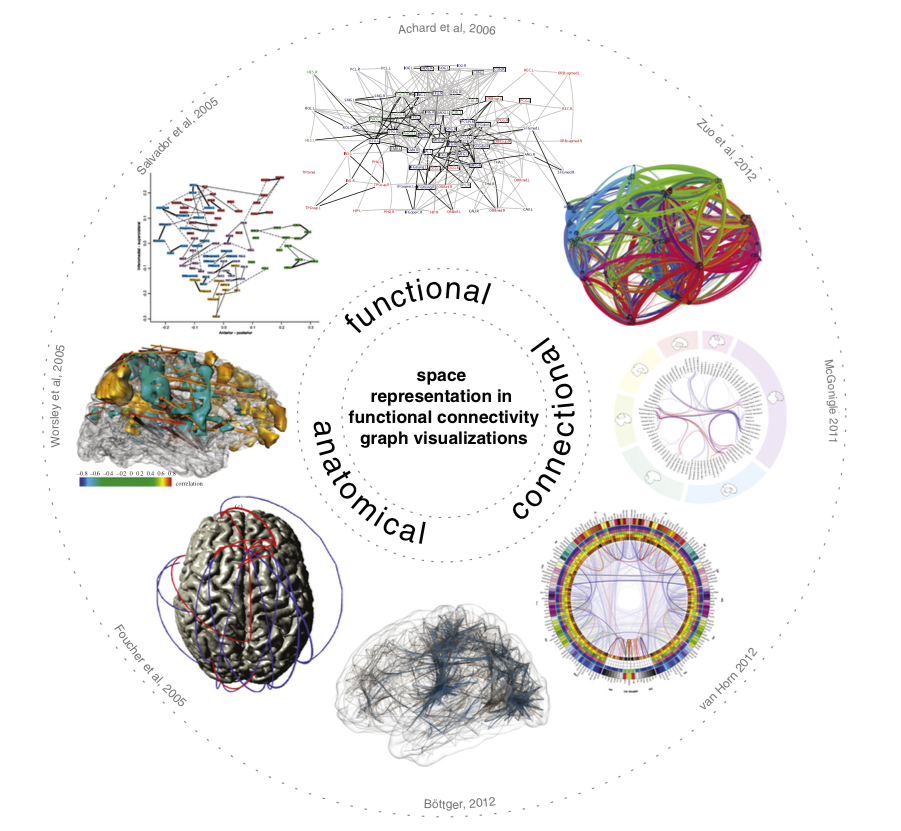
\includegraphics[width = 1.8\columnwidth]{taxonomy}
\caption{Taxonomy proposed in \cite{visualizingHumanConnectome} to group human connectomics visualization tools.}
\label{fig:taxonomy}
\end{figure*}
\section{Main Tasks}
\label{sec:mainTasks}

One of the worse mistake that can be done when designing a visual analytics tool is the willingness of addressing a spread set of tasks. Clearly understand what the main tasks are in a given research area is highly important. This activity it is not as simple as it might seem at a first glance. So, in this section I try to clarify and discuss the main goals neuroscientist would like to achieve using a human connectome visualization tool.\\

Due to the high complexity of the brain network, \textit{exploration} is the the most important task. Although some readers may argue that the exploration task is too simple, quite obvious and too general, in my opinion, it is not so. In fact, especially when the field is quite novel and with many uncleared aspects, as it is the one we are talking about, it is extremely relevant to allow to users a \textit{visualization flexibility}. Flexibility should be achieved in terms of level of abstraction, perspective and data that can be visualized. \\


\textit{Comparison} is the other task that should be achieved by a visual analytics tool. For example, neuroscientists are usually interested in comparing healthy and diseased subjects, so that it is possible to understand if there are different connectivity patterns in the two brain networks, which connections are missing and which are still active. For example, in studies like the one proposed by Bassett et al. in \cite{hierarchicalOrganization}, the authors show there are topological and connectivity differences in schizophrenic patients with respect to healthy subjects. Other works like \cite{alzheimer} have shown that in Alzheimer's disease some functional connectivity properties of healthy people are not present in diseased patients . So, having an easy-to-use visualization tool could accelerate this process and could hopefully allow more interesting discoveries in the field.

By interviewing neuroscientists, it emerged that dimensionality reduction methods, such as isomap \cite{isomap} and t-SNE \cite{tsne}, are frequently used. These methods allow to reduce the high-dimensional dataset in three-dimensions. The output of the mentioned techniques is addressed as \textit{brain intrinsic geometry} and the space in which it is plotted is called \textit{topological space}, as it is explained in \cite{bullmore2011brain} by Bullmore and Basset. So, experts not only are interested in looking at the brain anatomical structure, but also in the brain intrinsic geometry in a topological space. The idea behind this interest is that the brain could also hide some meaningful structural pattern in topological space.
%Then, not only experts are looking at the anatomical geometry of the brain, but also to what is often referred as  \textit{intrinsic geometry} or topological space as it is explained in \cite{bullmore2011brain} by Bullmore and Basset. Experts are looking for differences connectivity and structural patterns in healthy and diseased patients. In fact, experts in neuroscience want to understand if the organization of the brain network is nonrandom.
%In fact, after applying the isomap technique is possible to obtain what is also called the \textit{intrinsic geometry} of the input dataset, that, in this case, is the brain. So, experts are looking for connectivity and structural patterns in healthy and diseased patients. In fact, differences in two isomaps, using data from two different patients, can be caused by the structure of the geometry.  An intuitive and immersive visualization experience could help neuroscientist to explore and compare brain's data.

The last main task highlighted by experts is to find a way to inspect each dimension of the dataset collected. As we have said already, the brain's data are usually multi-dimensional one. Being able to inspect each dimension on the fly and choose the most meaningful ones to display would be the most important achievement in this field.
%
%\begin{figure*}[ht]
%	\centering     
%	\subfigure[3D Brain View]
%		{
%			\centering
%			 \label{fig:connections}
%			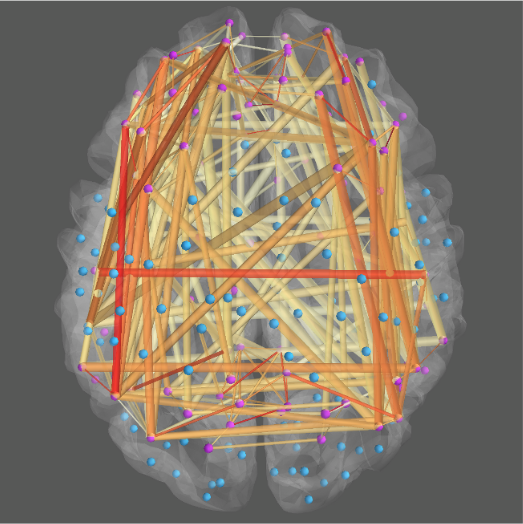
\includegraphics[width=0.6\columnwidth]{connections}
%		}
%	\subfigure[Circle View]
%		{
%			\centering
%   			\label{fig:circle}
%			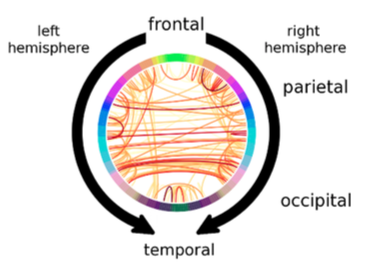
\includegraphics[width=0.6\columnwidth]{circle}
%
%		}
%	\subfigure[Matrix View]
%		{
%			\centering
%   			\label{fig:matrix}
%			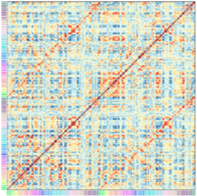
\includegraphics[width=0.6\columnwidth]{matrix}
%		}
%				
%	\caption{TODO!!!!!!!!!}
%\end{figure*}

\section{Survey}
\label{sec:survey}


% Node-link Comaprison Image


\begin{figure*}[ht]
	\centering     
	\subfigure[Connectome Visualization Utility]
		{
			\centering
			 \label{fig:nodeLinkConnectome}
			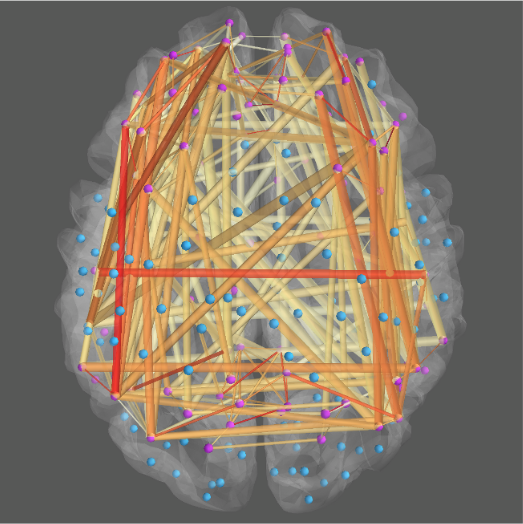
\includegraphics[width=0.6\columnwidth]{connections}
		}
	\subfigure[Brain Net Viewer]
		{
			\centering
   			\label{fig:nodeLinkBrainView}
			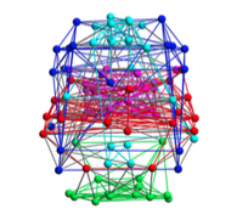
\includegraphics[width=0.6\columnwidth]{nodeLinkBrainView}

		}
	\subfigure[2D Node-link diagram]
	{
		\centering
		\label{fig:2DnodeLink}
		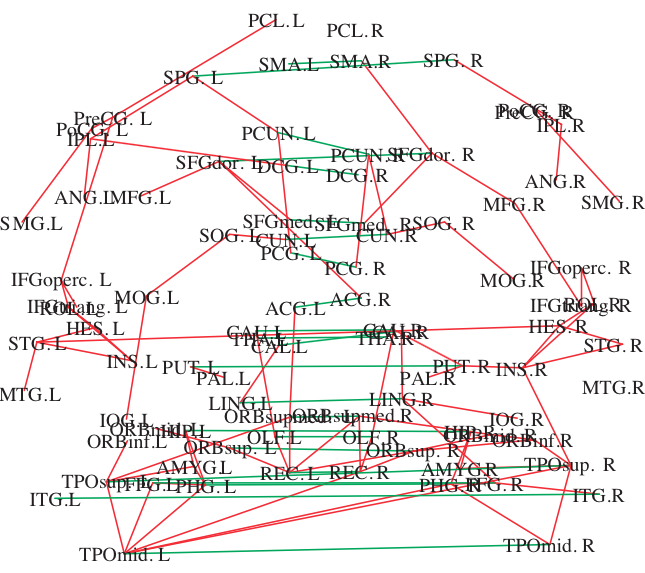
\includegraphics[width=0.6\columnwidth]{2D-NodeLink}
	}

	\caption{This figure groups the different views of node-link diagrams. In subfigure (a) there is the one provided by Connectome Visualization utility \cite{connectomeVisualizationUtility}. Subfigure (b) shows the visualization offered by Brain Net Viewer \cite{brainNetViewer}, while subfigure (c) presents the 2D flat view proposed in \cite{salvador2005undirected}.}
\end{figure*}


Many visualization tools have been presented in the academic literature, but, before describing them more in details, I would like to report the interesting taxonomy presented in \cite{visualizingHumanConnectome} by Margulies et al. In fact, they identified three main categories of visualization methodologies for the human Connectome: \textit{functional}, \textit{anatomical} and \textit{connectional}. The reasons beyond this taxonomy and its meaning are quite straightforward. In fact, visualization tools are clustered according to the common task they would like to face. Namely functional tools tend to privilege functional activity, anatomical tools visualize the brain itself using very often volume rendering techniques, while in connectional tools, visualizations are focused on the structural interconnections of the brain. Figure \ref{fig:taxonomy} gives an overview of the cited taxonomy. In the following subsections I will focus my attention only on connectional and functional methodologies. In these two categories there are three main approaches to represent the connectome precisely: \textit{node-link diagrams}, \textit{matrix-based diagrams} and \textit{circle views}. Then this section is structured as follows: firstly I am going to describe there three main approaches mentioned before, while in subsection \ref{subsec:weightedGraph} I will describe a interesting approach to compare weighted graphs and in subsection \ref{subsec:tractography} I will give an overview about tractography, namely the main approach to visualize DTI data.


\subsection{Node-link diagrams}
Node-link diagrams are one of the most used approach to represent graphs in general, and in particular to visualize the Connectome. The node-link diagrams could be based on 3D rendering or in a simple and flat 2D view. Recent visualization softwares like \textit{Connectome Visualization Utility} \cite{connectomeVisualizationUtility}, \textit{Brain Net Viewer} \cite{brainNetViewer} and \textit{Connectome Viewer Toolkit} \cite{connectomeViewer} provide this kind of 3D visualization. Usually, the dimension of the nodes is binded to some graph-based metrics, like nodal strength or nodal degree, while the weight of the edges is displayed using different colors or by changing diameter of the cylindrical link. Older studies on functional brain connectivity like the one proposed by Salvador et al. in \cite{salvador2005undirected}, instead, show a plain flat 2D node-link diagrams. Moreover, in this particular case, classical circular nodes are replaced by the name of the regions they stand for.\\ The main advantage of this approach is that it is possible to have a good overview of the entire graph and it is quite easy to understand which nodes are indirectly connected. With 3D rendering is also possible to give a spatial information and the tools locate the nodes following the real anatomical position. However, when the graph and the number of edges increase, the cleanness of the visualization is affected and the view becomes less intuitive and less understandable. Nonetheless, despite the usage of different dimensions to display the weight of the edges, their representation is not the most intuitive one. \\
Figures \ref{fig:nodeLinkConnectome}, \ref{fig:nodeLinkBrainView} and \ref{fig:2DnodeLink} collect the different visualizations offered by the three different tools above mentioned.


\subsection{Matrix-based diagrams}
\label{subsec:matrixbased}
The other well-known approach in graph visualization is the \textit{matrix-based} representation. Among all the software surveyed the only two of them which proposed this methodology are the Connectome Visualization Utility and the Connectome Visualization utility. The main advantage of this methodology is the clarity conserved when displaying information about relatively big graphs (more than 20-30 nodes). It is also effective the color encoding to display the weight of the links. However, this approach hides the information about the indirect connections there are between nodes. For this reason very often the matrix-based diagram and node-link diagram are combined together. In my opinion, the reason why only two tools proposed this approach is that people do not want to lose the spatial information embedded natively in the dataset usually collected. Although, in these tools it is possible to reorder columns and rows using the anatomical order and the alphabetical one. An example of matrix-based view is showed in figure \ref{fig:matrix}.
\begin{figure}[H]
\centering
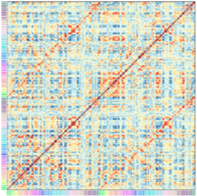
\includegraphics[width = 0.9\columnwidth]{matrix}
\caption{The matrix-based diagram proposed in \cite{connectomeVisualizationUtility}. Columns and rows represent the regions, while a color encoding is used in the cells to represent the weight of the edges.}
\label{fig:matrix}
\end{figure}


% Circle Views Compared

\begin{figure*}[ht]
	\centering     	
	\subfigure[Irimia et al. \cite{irimia2012patient}]
		{
			\centering
   			\label{fig:circleIrimia}
			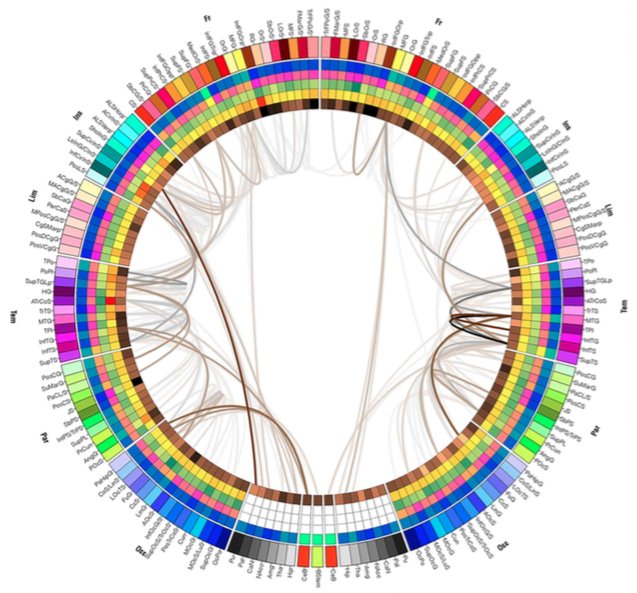
\includegraphics[width=0.95\columnwidth]{circleIrimia}
		}
	\subfigure[Connectome Visualization Utility]
		{
			\centering
			 \label{fig:circleConnectome}
			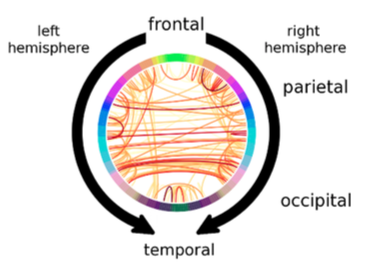
\includegraphics[width=0.95\columnwidth]{circle}
		}
	\caption{This figure put in comparison the two \textit{connectograms} described in sections \ref{subsec:circleviews}}
\end{figure*}

\subsection{Circle Views}
\label{subsec:circleviews}
A quite innovative representation is the one very often addressed as \textit{circle view} or \textit{connectograms}. This kind of view was firstly introduced by Irimia et al. in \cite{irimia2012patient} in 2012. A circle view has been also re-proposed in the Connectome Visualization Utility \cite{connectomeVisualizationUtility} two years later.
With circle view, all the regions are displayed along a circle and the interconnections are represented as edges that go from region to another inside the circle. Quite effective is the usage of transparency to represent the weight of the edges in \cite{irimia2012patient}. The transparency reduces the visual disorder and attract the user attention only on strong links, while weak edges fade into the background smoothly. The connectograms, showed in figure \ref{fig:circleIrimia}, contains six nested circles. The outermost circle represents the cortical parcelations, while the five innermost circles are heat maps which display five different structural measures associated with the corresponding regions.\\
The Connectome Visualization Utility allows two ways of organizing the position of the regions. In fact, it is possible to order them according to their names (alphabetically) or according to the real position in the brain as it is shown in figure \ref{fig:circleConnectome}. \\
This approach is quite effective and clear even with the increase of the number of edges and nodes. Still, the heat maps can be ineffective especially when the number of nodes becomes bigger. The main drawback of this technique is the static nature of the visualization. At the moment I am writing, there are no implemented examples of dynamic and interactive connectograms.






%\subsection{Still unnamed}
%The Connectome Visualization Utility \cite{connectomeVisualizationUtility} is one of the main tools available in the literature to visualize the human brain connectiontivity. To visualize the Connectome the authors propose three different kinds of visualization approaches: 3D brain view, circle view and matrix view.\\
%In \textbf{3D Brain View} the brain surface is depicted on the screen and nodes are located according to the physical position in the brain itself. The many connections present in the brain are represented as edges in the brain. This view is interactive and it is possible to isolate all the connections that starts from a selected node. Figure \ref{fig:connections} shows this view.
%
%
%
%
%With \textbf{Circle view} all the regions are displayed along a circle. The connection between all the nodes are represented as edges that go from region to another inside the circle. There are two ways of organising the position of the regions. In fact, it is possible to order them according to their names (alphabetically) or according to the real position in the brain as it is shown in figure \ref{fig:circle}.
%
%The \textbf{Matrix view} represents the entire network using the adjacency matrix. Nodes are positioned along the sides of a square matrix. Using colors each cell represent how strong the connection between two nodes is. Still in this view, it is possible to order the nodes alphabetically by their names or by the anatomy. Figure \ref{fig:matrix} shows this kind of view.\\
%
%
%In the last two views the order in which the regions are displayed has a relatively big influence on the visualization itself. \\
%An interesting characteristic of these tool is the chance to bind the size of the spheres, which represent the brain regions, to some graph metric such as nodal strength or nodal efficiency. This is a very interesting functionality since experts could understand in a very straightforward way some nodal measures computed on the overall network.\\


\begin{figure*}[ht]
\centerline{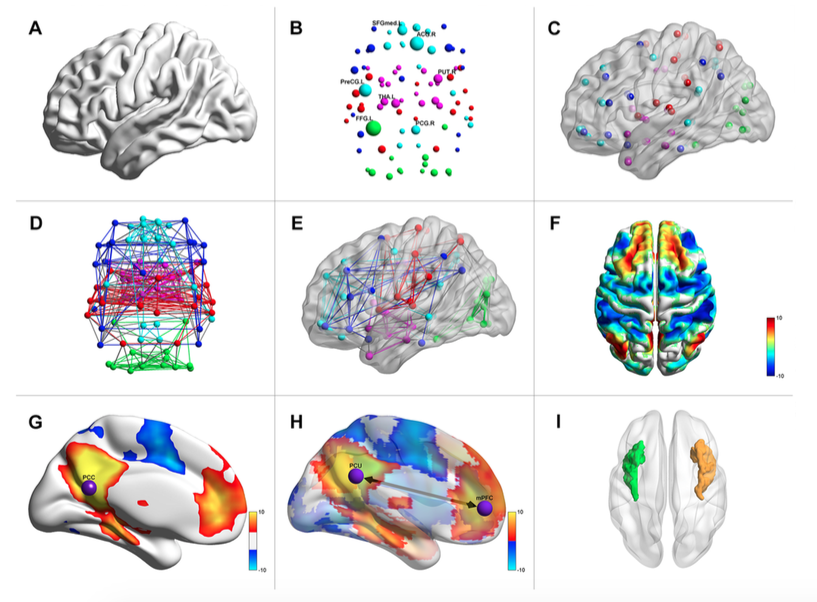
\includegraphics[width=1.9\columnwidth]{brain2}}
\caption{Some screenshots taken from Brain Net Viewer \cite{brainNetViewer}. The tool also allows to contextualize the node-link diagram with a 3D brain model.}
    \label{fig:brain2}
\end{figure*}

%\begin{figure*}[ht]
%\centerline{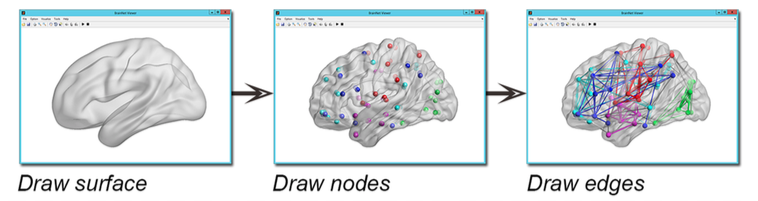
\includegraphics[width=1.9\columnwidth]{brain1}}
%\caption{This figure represent the three possible ways in which it is possible to represent the brain Connectome.}
%    \label{fig:brain1}
%\end{figure*}


%\subsection{TODO: FIND A NAME}
%BrainNet Viewer \cite{brainNetViewer} is a visualization tool for human brain connectomics. This tool provides many visualizations using a ball-and-stick model. So, each visualization is composed by nodes that are representing brain regions and sticks which represent the connections between the regions. Moreover, BraiNet can display also the brain surface. Each combination of these three elements (nodes, edges and surface) can be displayed according to the user choices.\\
%The dimension of the nodes can be linked to some measures performed on the network such nodal strength and nodal efficiency, but it still unclear what the degree of freedom is given to the user. Both structural and functional networks can be visualized thanks to this tool.\\
%The most interesting feature this tool provide is the possibility to show the brain surface and the connectome at the same time. Another feature that appears in this tool, which is unfrequent in connector visualization tools, is the possibility to color edges according to their distance. Thanks to this, it has been possible to see that, in the vast majority of the cases, long connections link homologous regions in the two different hemispheres. Figures \ref{fig:brain2} and \ref{fig:brain1} show some screenshots from the working tool.




\subsection{Weighted Graph Comparison}
\label{subsec:weightedGraph}
\begin{figure*}[ht]
\centering
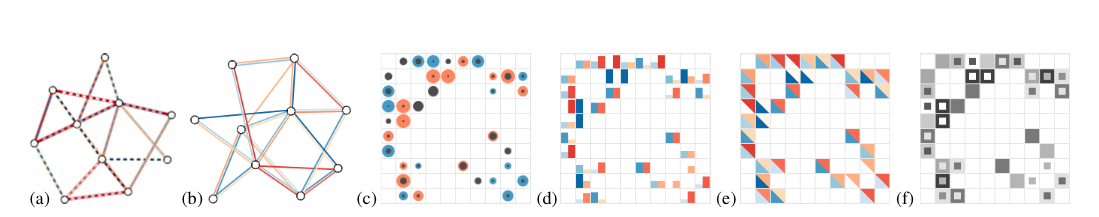
\includegraphics[width = 1.8\columnwidth]{weightedGraphs}
\caption{The prototypes proposed by Arper et al. to easily compare weighted graphs. The first two images represents node-link diagrams, while the remaining four are different versions of matrix-based representations. Images taken from \cite{weightedGraphComparison}.}
\label{fig:weightedGraph}
\end{figure*}

In 2013, a very intriguing study has been introduced by Alper et al. in \cite{weightedGraphComparison}. The problem they addressed was to find the right visualization when comparing weighted graphs. Although this is a wide issue related to graph visualization in general, the authors focus their attention on the graphs derived from the connectome studies. To achieve the goal briefly described before, the authors proposed two main techniques: matrix diagram and node-link diagram. With the matrix diagram each cell represents the weight of the link using a brightness encoding. The other methodology is the node-link diagram in which all the edges are drawn. If an edge is present in both of the adjacency matrices, there are two edges as well and the higher weight has a brighter color. When just one edge is drawn, it simply means that a connection is missing in one of the two graphs. Figure \ref{fig:weightedGraph} shows the prototypes proposed by the team.\\
The paper reports also a very strong validation process in terms of people involved (11 participants) and metrics measured. They registered many different metrics and the results are quite interesting. Conversely to what people may think, the matrix diagrams revealed to be more effective than node-link diagrams are. That is a very important and novel result, since it is the first comparison tool I have seen in the literature and the result is not intuitive. It would be interesting to go further in this study and try to have a study with more participants.\\
The most impressive design decision is that a 3D visualization has been excluded a priori since the authors claim that "the clutter and complexity of the visual encoding in these spatial/volumetric representations makes it difficult to perform accurate weighted edge comparison tasks". Moreover, writers state that the vast majority of neuroscientific tasks can be fulfilled using a 2D representation and that the third dimension could be misleading in the interpretation. This is a quite strong statement and follows the idea Tamara Munzner has about the third dimension presented in \cite{processAndPitfalls}. She claimed that the third dimension should be strongly motivated, because it is not true that having three dimensions is always better than having just two of them. Although the paper presents a strong validation process, it is not clear why the authors decided to use just synthetic data instead of real dataset, even though connectome data are easily available. The idea of creating a specific visualization technique to compare weighted graph is quite novel and the results are interesting as well. The weakest part of the study was the choice to use artificial datasets, instead of real ones. Although the evaluation choice may raise some doubts, they certainly opened a new challenging research topic.

\subsection{Tractography}
\label{subsec:tractography}
Tractography is a technique to represent data collected from diffusion MRI, also addressed as Diffusion Tensor Imaging (DTI). DTI dataset contains measure about the motion of water molecules in brain tissues. Since the brain white matter is a fibrous structure, water molecules diffuse more in the directions along the fibers rather than on the perpendicular dimension. This kind of movement is called \textit{anisotropic}, in contrast with the \textit{isotropic} diffusion of water molecules when they can freely move in the space. Thanks to this anisotropic movement it is possible to reconstruct the fiber presence and orientation. Then, using tractography is one of the most common way to go back to these informations. This reverse process is quite hard also because DTI dataset are multidimensional. In fact, when performing DTI it is possible only to see that good diffusion exists along the direction in which a gradient is applied. So if we want to know the diffusion in all directions, we should get many diffusion weighted images with gradients in different directions. In principle, 'all directions' would mean every possible direction on a sphere, but in practice 12, 16, or 32 gradient directions (or more) are considered. DTI data contains by design some uncertainty, just because it is not possible to scan all the possible directions in a 3D space. However, finding a way to represent the embedded uncertainty in the data is quite hard. The need of a representation makes the researcher coin the word \textit{deterministic tractography}. Researcher just cleared any ambiguity by describing connections with a concrete tract \cite{conturo1999tracking}, \cite{mori1999three}. 

\begin{figure}[H]
\centering
\includegraphics[width = 0.8\columnwidth]{hairLike}
\caption{The hair-like structures tractography proposed by Peeters et al. in \cite{peeters2006visualization}}
\label{fig:hairlike}
\end{figure}

More recently with the emergence of computer graphics, new advanced methodologies following the same trend aforementioned came out. So, tracts have been represented with \textit{tuboids}\cite{petrovic2007visualizing}, \textit{hair-like structures} \cite{peeters2006visualization} and \textit{stylized line primitives} \cite{stoll2005visualization}. In 2012, a work written by Congote et al. proposed a web-based application to render tractography \cite{congote2012real} with a real-time volume rendering technique. \\
As well as deterministic tractography has been the main topic in different academic works, many researchers focused their attention on finding an effective way to deal with the intrinsic uncertainty embedded in DTI. Many visualizations, able to englobe the variability of the data, and error-reduction techniques have been proposed, but this topic is out of the scope of this work. Figure \ref{fig:hairlike} shows the hair-like tractography, while figure \ref{gig:realtime} presents a real-time volume rendering approach.


\begin{figure}[H]
\centering
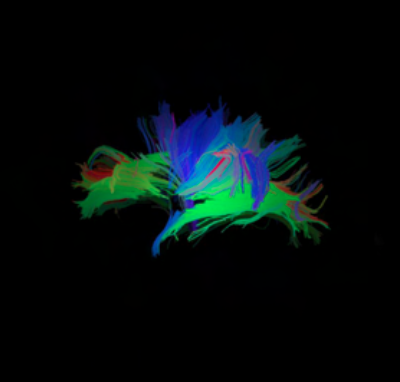
\includegraphics[width = 0.8\columnwidth]{realTimeTractography}
\caption{Tractography displayed using real time volume rendering approach proposed by Congote et al. in \cite{congote2012real}}
\label{gig:realtime}
\end{figure}


\section{Future Works and New Trends}
\label{sec:futureWorks}
Although all the methodologies proposed are quite interesting and the results may have a very positive impact on experts exploraration, still all of these visual analytic tools are affected by a lack of portability between platforms and the methods used are not usually described in a replicable manner. The applications have been written with a variety of languages that go from Matlab to Python, so they can be considered \textit{stand-alone} and \textit{local} applications. However, in the last few years the clear trend in computer science is to move all the services to the web. There are many reasons why we are witnessing this process. Among them I would like to remind the flexibility, cross-platform native feature and, not least, the higher and higher computational power that newer browser can support. This field is also shyly moving towards this kind of technology and web-based application. To this regard, the javascript library \textit{Xtoolkit} \cite{xToolkit} has been created to drive this natural flow. XToolkit is a framework its aim is to allow Javascript web-based visualization tools and it claims to be a "lightweight and fast" webGL framework for scientific visualization. Apart from wrapping many webGL functions, the main contribution offered by this tool is the possibility to read and load standard neuroscience file extensions. On the top of this framework, tools like Brain Browser \cite{brainBrowser} have been created. \\

At the same time, the human connectomics visualization is moving from 2D space to a 3D one. Although there are no well-defined examples or complete applications that use 3D modeling, still this transition seems to be the right path to follow. In fact, the last tools I have introduced before not only are changing the technology, but also are trying to use the potentiality of 3D to render in a more effective way the human brain Connectome. Still, those example are primitive, the interaction is limited and, at the moment, can not be compared to more established and complex visual analytics tools like the ones described in section \ref{sec:survey}.\\
A very recent paper published by Arsiwalla et al. \cite{arsiwalla2015network} has introduced a virtual reality visual analytics tool for the Connectome. This enforces that the path towards an immersive virtual reality is the one researchers are mostly focusing on. 


\section{Conclusions}
\label{sec:conclusions}

The work surveyed and summarized the main techniques and methodologies used to visualize human connectomics as well as highlights the new ideas that can be followed for future works. This research area is quite novel that is why there are just few complete visualization tools able to deal with the data collected. Still, these tools are quite complete and had a positive impact on the neuroscientist community. The main drawback is the lack of portability which affects all the tools described and that is why we are seeing a transition towards more flexible and cross-platforms technologies such as \textit{Javascript}. Moreover, 3D rendering can be exploited much more and a researchers came out with the idea of using immersive virtual reality.


\bibliography{mybib}{}
\bibliographystyle{plain}  




%------------------------------------------------

\end{multicols}
\end{document}